\chapter{Experimental Setup}
\label{chp:experimental_setup} 

intro..

\section{Microphone selection}\label{sec:ch3_microphone_selection}

In our project, we use different kinds of experimental setups. 
The first setup is the Zoom H4n Handy Recorder. 
The recorder is able to record WAV files with a sampling frequency \( {F_{s}} \) of 96kHz and a quantization of 24 bit. We were also able to plug it directly into a computer, thus using it as the standard sound input device. 
However this limited the operating sampling frequency \( {F_{s}} \) to 48kHz.

To be able to record even higher frequencies, we use a Knowles Ultrasonic microphone connected to a National Instruments myDAQ device. 
The microphone should be able to detect frequencies up to 100kHz combined with the myDAQ that is able to sample with a \( {F_{s}} \) of 200kHz.

Since a lot of the information we are looking for is in a frequency range far above the hearing range of the human ear, we require a microphone that can capture these frequencies. 
The frequencies we are able to observe are limited to the Nyqyust frequency.

\begin{equation}\label{eq:ch3_nyquist_frequency}
F_{nc} = \frac{F_{s}}{2}
\end{equation}

This means that we are able to study the frequency response up to frequencies of 48kHz using the setup.
In original research, it is claimed that there is information for fingerprinting in this frequency range, thus we should be able to observe the phenomenons.

\subsection{Zoom H4n Configuration}\label{sec:ch3_zoom_H4n_configuration}

The Zoom H4n Handy Recorder is set to Sterio Mode.
Further, the sampling frequency is set to 96 kHz and the analog to digital converstion is set to the maximum which is 24 bit.
The recorder provides a 237 Hz low cut filter, which is enabled.
These low-frequency frequency responses are not providing information that is critical for looking at the fingerprints and \todo{citation paper; Look at explanation from the original paper} \todo{Low cut filter not working??? Cannot be observed in plots ...} 

Since we do not have a remote controll for the recorder, we have to manually click the record button to start and stop our recordings. 
This means that we are touching the recording device, thus impacting the samples when the contact is happening. 
This is not critical for our setup, as we are recording a time interval of several seconds; only the samples in the timeframe when we are activly starting and stopping the recording are affected by the physical contact. 
However this makes it harder for us to do multiple recordings with the recorder in the exact same place, as touching the device will inevitably cause some slight displacement.

\subsection{Knowles Ultrasonic SPU0410LR5H Configuration}\label{sec:ch3_knowles_configuration}

The Knowles Ultrasonic SPU0410LR5H microphone is able to detect sound up to 80kHz with a -4dB sensitivity\cite{knowles_spec}. 
To be able to record frequencies up to 100kHz, we need the National Instuments myDAQ to sample the sound at a \( {F_{s}} \) of 200kHz.
The microphone is connected to a 4.5V battery and directly in to Analog Input 0 on the myDAQ device. 
The myDAQ device has a buildt in gain of ?? \todo{find out how much}, which is enough for us to enterpretate the signals.

\begin{circuitikz} 
  \draw (3,0) node[op amp] (opamp1) {}
  (opamp1.+) node[left ] {1-40mV $v_+$}
  (opamp1.-) node[left ] {$v_-$};
\end{circuitikz}



\begin{figure}[h]
    \centering
    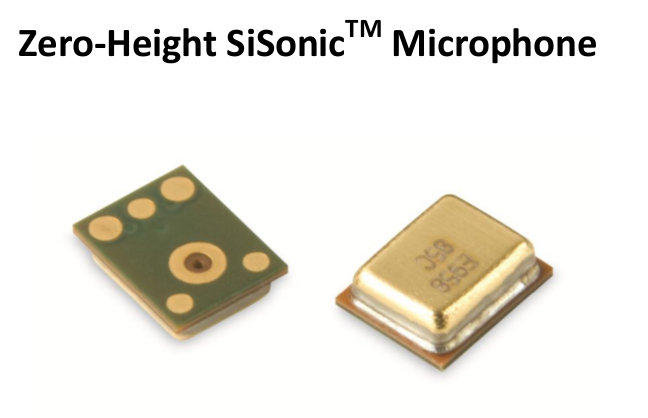
\includegraphics[scale=0.3]{knowles_microphone.png}
    \caption{Knowles Ultrasonic SPU0410LR5H}
    \label{fig:knowles_microphone}
\end{figure}




\section{Processing and signal extraction}\label{sec:ch3_processing_signal_extraction}

The captured sound is stored in a WAV file.
This file is processed in our self written software, which utilizes libraries such as FFTW \todo{citation here} and libsndfile \todo{citation here}.
The samples are devided into windows \( W \), where \( \lvert W \rvert = 2^{n} \) where \( n \) is a non-zero positive integer.

The WAV file contains a sterio signal, but since our audio source is hardly a sterio source, we only need one of the channels for our furter processing. \todo{Reasoning about why we only need mono} In the WAV format, frames representing each sample is stored subsequently, such that the sample \( s_{f,c} \) represents the PCM \todo{Pulse-code modulation abbrevation} response for frame \( f \) channel \( c \). Since we have a stereo signal, we have that \( f \in \left [ 1, 2 \right ]  \), and thus the samples are ordered  \( s_{0,0}, s_{0,1}, s_{1,0}, s_{1,1}, ... , s_{n,0}, s_{n,1} \). To obtain a mono signal we simply ignore all frames where \( f \neq 0 \).


\section{Capturing audio fingerprint}\label{sec:ch3_capturing_audio_fingerprint}

1. 
Type: Micro ops
Microphone: Knowles SPU0410LR5H
Mic position: Above CPU
Computer: Lenovo T60p

2. 
Type: RSA decryption
Microphone: Knowles SPU0410LR5H
Mic position: Above CPU
Computer: Lenovo T60p

3.
Type: RSA decryption
Microphone: Knowles SPU0410LR5H
Mic position: Outside fan
Computer: Lenovo T60p

4. 
Type: RSA decryption
Microphone: Zoom H4n
Mic position: Above CPU
Computer: Lenovo T60p

5. 
Type: Micro ops
Microphone: Zoom H4n
Mic position: Above CPU
Computer: Lenovo T60p